\chapter{Results} \label{ch:results}

In this chapter we analyse models regarding their feature distribution and algorithms regarding their performance.
Furthermore, we investigate which model-features have influence on the performance of the algorithms.

Regarding runtime a lot of stuff may change. Iterations wont change as long as we use the same deterministic algorithms, so its a more stable metric.

Various studies we have made, knit into a nice purple string and story. Here might appear:
Maybe it would also be cool to show preformance differences in real case studies in comparison to the random generated models and make conclusions Ideally:
\textcolor{purple}{We did previously not have enough models to see behaviour XYZ but now we can.}

\section{Experimental Setup}
Various algorithms we consider were already implemented in PRISM-games~\cite{prismgames3}.
We needed to extend PRISM-games by the algorihtms $\LPSI$, $\TLPSI$ and $\TOPAlg$.
Moreover, for $\TOPAlg$ we added precise Markov chain solving, which was not present in PRISM-games before and extended the strategy iteration (which was implemented in~\cite{gandalf20}) to use this precise solving.
Our code is available in the github repository \url{https://github.com/ga67vib/Algorithms-For-Stochastic-Games}.

\subsubsection*{Technical details}
We conducted the experiments on a server with 64 GB of RAM and a 3.60GHz Intel CPU running Manjaro Linux. %Intel (R) Xeon(R) W-2123 CPU.
We always use a precision of $\varepsilon=10^{-6}$. The timeout was set to 15 minutes for all models. 
The memory limit for every experiment was 6 GB.

\section{Model Analysis Results}

First, we want to learn about the feature-distribution of the real case-studies we have. For this we use a box plot for each feature.
\textcolor{purple}{Most likely I may move all the features into the appendix and only highlight 5-10 cool features.}
\begin{figure}[t]
    \centering
    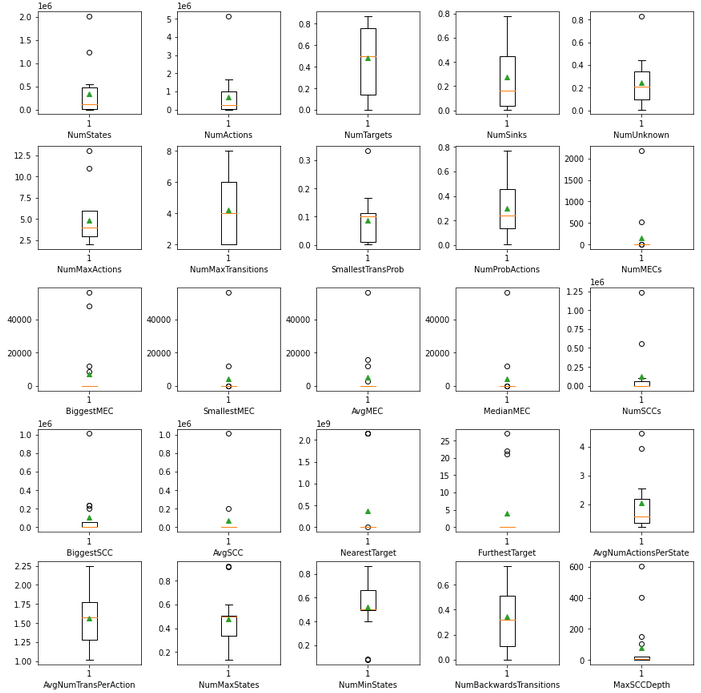
\includegraphics[width=1\textwidth]{figures/Real_FeatureDistribution.png}
    \caption[Feature Distribution of the case-studies]{
        Box-plot of the feature distribution of the real case-studies.
        In each graph, the distribution of the values of one separate feature over all real case studies is visualized. 
        The orange line marks the median of a feature over all models and the green triangle marks the average.
        The bounds of the boxes mark the 25 and 75 percentile, and the lines extended by the whiskers mark the 10 and 90 percentile.
        \textcolor{red}{Not sure about the 10 and 90 percentiles}
        Dots outside of whiskers represent outliers.
        The relative number of probabilistic actions for example is between around $15\%$ and $45\%$ in half of the models.
        In half of the models, more than $20\%$ of actions are probabilistic.
    }
    \label{fig:Real_FeatureDistribution}
\end{figure}
What we can read from the box plot is this:
\begin{itemize}
    \item Models have around 2 actions per state and 1.5 Transitions per action
    \item Some of our models were trivial
    \item A huge part of the models is actually trivial
    \item Generally, the number of states is evenly split to Maximizer and Minimizer
    \item Usually, around 70 to 85\% of all actions are deterministic
\end{itemize}

By furthermore printing the maximal and minimal ocurring values of each feature we obtain that the smallest ocurring positive transition probability is 0.001.

With this information we can draw conclusions about which structural cases do not appear in the real case studies. 
None of the models contain these cases:
\begin{itemize}
    \item Models with a large number of actions per state
    \item Models with a large number of Transitions per action
    \item Models with very small transition probabilities like 1e-6
\end{itemize}

We can also use boxplots to assess whether our random-generation procedure favours some feature-values over others or is uniformly distributed.
\begin{figure}[t]
    \centering
    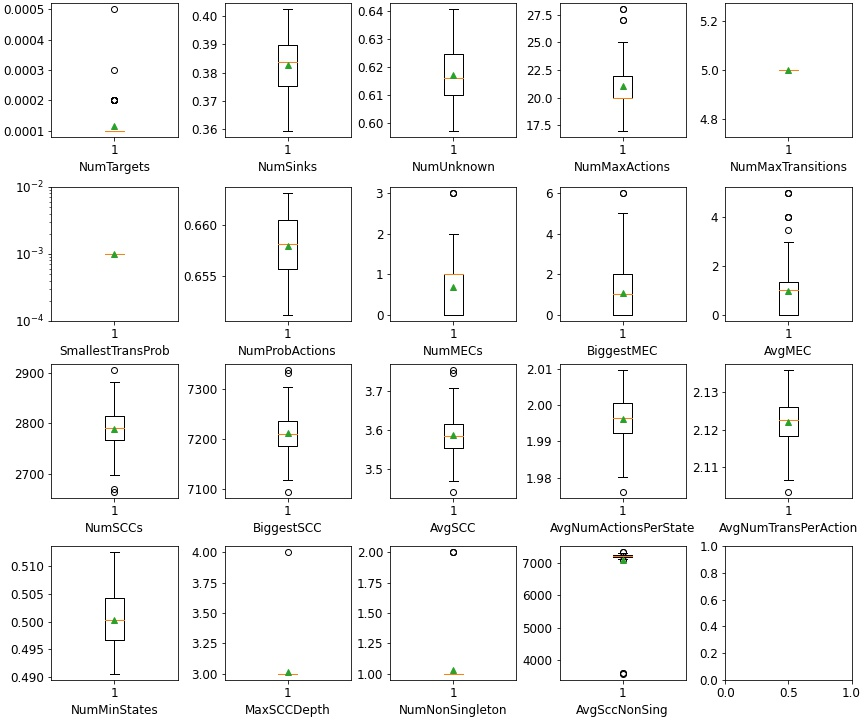
\includegraphics[width=1\textwidth]{figures/RandomRandom_FeatureDistribution.png}
    \caption[Feature Distribution of random models]{
        Feature Distribution of random models
    }
    \label{fig:Random_FeatureDistribution}
\end{figure}

The insights we generate from this are:
\begin{itemize}
    \item We have raised the number of unknowns on average to 30\% in comparison to the 20\% of the real data set. As seen from NumSinks, almost all known states are sinks.
          This is because we can have both trivial and non-trivial minimizer MECs that operate as sinks.
          We could try to remove them, but then we would intervene with the random nature of the procedure.
    \item As mentioned in Chapter \ref{ch:randomGen}, our procedure generates models with a tendency to having few actions per state and few transitions per action.
    \item The rest of the current image is very dependent on the parameters we set, so it pointless talking about it.
          Or we could use is as example.
          \textcolor{red}{However, I should create 100 models with the same parameters and then see their feature distribution of non-set features.}
\end{itemize}

\section{Algorithm Analysis Results}

In this section, we compare various prominent algorihtms and their optimizations on real case studies, handcrafted examples and our randomly generated models
to 

Overall, we compare the following algorithms:
\begin{itemize}
    \item $\VI$: Value iteration with naive stopping criterion
    \item $\BVI$: Bounded value iteration providing a guarantee \cite{paperMaxi}
    \item $\OVI$: Value iteration with upper-bound guessing \cite{What?}
    \item $\WP$: Bounded value iteration with the widest path approach for the upper bound \cite{widestPath}
    \item $\LPSI$: Strategy iteration with linear programming as MDP solution technique
\end{itemize}

Additionally, we use optimizations on these algorithms that we also evaluate in our benchmarks. These are:
\begin{itemize}
	\item G: The Gau{\ss}-Seidel variant of value iteration for $\BVI$ and $\OVI$.
	\item D: The idea from~\cite{KKKW18} to only deflate every 100 steps for $\BVI$.
	\item T: The topological variant of $\BVI$, $\OVI$ and $\LPSI$.
	\item $\TOPAlg$: The precise variant of topological value iteration.
\end{itemize}

\subsubsection*{Case studies}
We consider case studies from three different sources: 
(i) all real case studies that were already used in~\cite{gandalf20}, which are mainly from the PRISM benchmark suite~\cite{PRISMben}. We omit models that are already solved by pre-computations.
(ii) several handcrafted corner case models: haddad-monmege (an adversarial for value iteration from~\cite{haddadmonmege}), BigMec (a single big MEC) and MulMec (a long chain of many small MECs), the latter two both being from~\cite{gandalf}.
(iii) randomly generated models generated by Algorithm \ref{algo:randomRandom} and our additional guidelines from Subsection \ref{sec:guidelines}.


\subsection{Comparing Algorithm-Performance}
First, we provide a general overview of the performance of all algorithms on our benchmarking set.
We do this by providing a fancy graph that I have copied from Maxi. \textcolor{purple}{I should also steal his description}

\textcolor{purple}{Should make the both plots in jupyter next to each other. This gives best quality screenshots. If not possible then at least make the height smaller}
\begin{figure}
    \centering
    \subfloat[\centering Performance Overview on real case studies]{{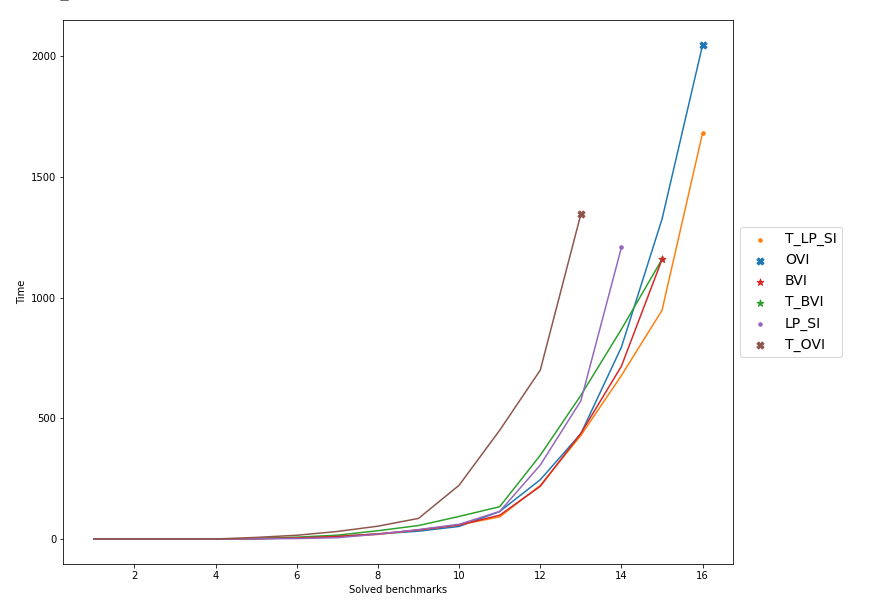
\includegraphics[width=0.8\textwidth]{figures/Real_AlgoPerformance.png} }}%
    \qquad
    \subfloat[\centering Performance Overview on random generated models]{{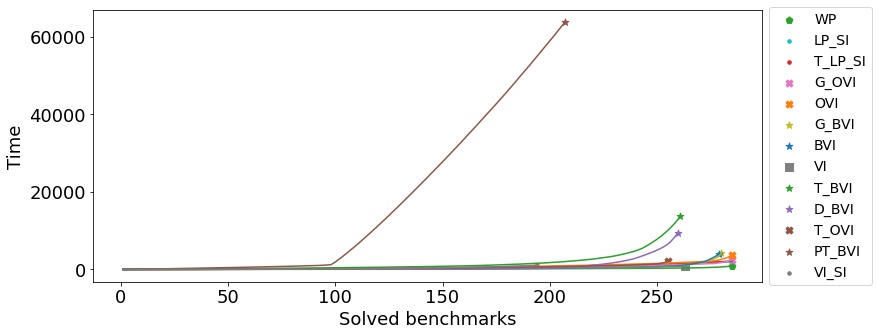
\includegraphics[width=0.8\textwidth]{figures/RandomRandom_AlgoPerformance.png} }}%
    \caption[Overview of Algorithm Performance]{Overview of Algorithm Performance}%
    \label{fig:AlgoPerformance}
\end{figure}

\textcolor{purple}{We also should do the same thing with iterations!}

What we can read from the graphs:
\begin{itemize}
    \item $\TLPSI$ is accumulated better than $\LPSI$.
    \item $\TLPSI$ is very good.
    \item $\LPSI$ good on random but not so good on real. Why?
    \item $\WP$ is usually the best value iteration approach
    \item $\OVI$ is usually better than $\BVI$ for small models
    \item $TOP$ does not seem very promising. We will find out why in the scatter plots
    \item The optimizations do not seem to do much except for the topological switch for $\TLPSI$ and $\WP$
    \item Why GBVI is not always better than BVI (iterationwise)
\end{itemize}

We investigate these clues by using more specific graphs.

\subsubsection*{Topological extension for strategy iteration with linear programming is usually benefitial}
\textcolor{red}{Show Scatter. Should usually be better. 
Maybe would be cool to do the same for OVI and BVI and show that there this is not the case. However, for that we may also point to GANDALF}

\subsubsection*{Topological strategy iteration with linear programming performs is good}
Altough value iteration is usually regarded to be the most performant algorithm type for solving stochastic games, 
$\TLPSI$ yielded the results alongside widest-path bounded value iteration.
Since strategy iteration simply tries to make an informed decision on which strategy to pick and solves the underlying MDP, 
we have to inspect the algorithms we use to solve MDPs - for $\TLPSI$ this is linear programming.

Although linear programming is believed to perform worse than value iteration for MDPs \cite{ANYTHING?},
we could not find clear superiority of value iteration on the reachability benchmarks for MDPs provided on \cite{QComps}.

Lastly, it is believed that linear programming scales worse than value iteration for huge models. But even if that is true,
$\TLPSI$ may be a good complementary solution approach in case a model is especially hard for value iteration.
Also, the topological improvement allows to solve models with huge numbers of SCCs faster than value iteration.
\textcolor{purple}{And also value iteration was the focus of research for the last 20 years. 
It is very likely that LP could be improved. Atm we do not even deflate but use MIP to encode the maximum-best-exit-constraints. But this should maybe go into future work}


\subsubsection*{Comparing OVI and BVI}
We use scatter plots, where every point describes the runtime of BVI in relation to the runtime of OVI to solve the model.

\textcolor{red}{Show here OVI and BVI compared. Iterations and Runtime. And also Real and Random. Its a 2x2 Graph. May also overlay random and real}

Clearly, OVI performs time-wise better than BVI. This does not hold true for the iterations. However, the most time consuming part of OVI is the deflation, of which OVI requires less.
\textcolor{red}{However, for big models an additional failed verification phase can be detremental for OVI. We should be able to see this in the big models. So I would probably not even recommend it.
This also shows the need for big models + BVI is an anytime approach}


\subsubsection*{Comparion Vanilla to Optimization Switches}
No big difference. Enter into the scatter plot both at the same time

\subsubsection*{Problems with TOP}
TOP seems to perform worse than vanilla in general. This is because we solve the DTMCs with exact methods, 
requiring a matrix inversion, which is $\mathcal{O}(n^{2})$-operation, where n is the number of states in the Markov Chain.
However, using iterative methods to solve the DTMC may yield better results. We have also tried MDP-LP-solving instead of MDP-SI-solving, but it was
still worse than $\TLPSI$.

\subsubsection*{Gauss-Seidel BVI}
Generally less iterations, but matrix operations of vanilla is faster.
Can sometimes be worse due to unlucky SCCs based on lower bound. Then the upperbound can fall behind the vanilla-upperbound
GS-bvi along topological enumeration of states could be better, check the results...

\subsection{Searching Correlations between Algorithms and Features}
Next, we are interested in  correlations between algorithm-performance and values of features.
Ideally, we would like to find cases where one algorithm scales better with certain features than others.
This would allow to analyse the graph structure and decide based on the features we get which algorithm is most likely the best one to use in this case.
To find these correlations, we use the following visualization tools:

\subparagraph*{Heatmaps}
Heatmaps visualize correlation matrices - matrices where one feature is mapped against another. The higher the correlation value, the stronger
a correlation between two features is. On the diagonal of the matrix the correlation is maximal since there is a directly proportional correlation between
a feature and itself. Ideally, we would like to get clues from the heatmap which features or correlations we should investigate.
However, for the most part we could not gather any non-trivial information from heatmaps.

\subparagraph*{Scatter Plots}
We plot algorithm runtime / iterations against feature values. Each point corresponds to the feature-value and runtime of a model.

What is there to find in these graphs?
\begin{itemize}
    \item Clearly visible how TOP scales with SCC-size
    \item All scale with number of unknowns, which is no surprise but might be mentioned.
\end{itemize}

\subparagraph*{One Dimensional Graphs}
We can get models where proposition A is fulfilled and compare them to models where A is not fulfilled.
We can plot the models where A is true against models where A is false to see whether they hold structural differences.
This did not seem to be the case in general.